%%%%%%%%%% DOCUMENT STUFF %%%%%%%%%%

\documentclass[11pt,letterpaper]{article}
\usepackage{mathtools}
\usepackage{amsmath}
\usepackage{amssymb}
\usepackage{datetime}
\usepackage{setspace}
\usepackage{tkz-graph}
\usepackage[margin=1in]{geometry}

%%%%%%%%%% FORMATTING %%%%%%%%%%

\newdate{date}{15}{02}{2017}
\date{\displaydate{date}}
\doublespacing
\setcounter{secnumdepth}{0}
\newcommand\tab[1][1cm]{\hspace*{#1}}

%%%%%%%%%% CONTENT %%%%%%%%%%

%%%%% COVER PAGE %%%%%

\begin{document}
\title{CS 180: Homework 3}
\author{
	Jonathan Woong\\
	804205763\\
	Winter 2017\\
	Discussion 1B}
\maketitle
\pagebreak

%%%%% PROBLEM 1 %%%%%

\section{Problem 1}
Given a sequence of requests with start and finish times $(s(i),t(i)) = 1, \dots , n,$ find a set of non-conflicting jobs of maximum possible size. Show that the following algorithm solves the problem correctly: \\
LATEST START TIME (LST): \\
(a) Set $R \leftarrow \{1,\dots,n\},$ and $A \leftarrow \emptyset$. \\
(b) While $R \neq \emptyset$: \\
\tab i. Pick request $i \in R$ with the latest start time. \\
\tab ii. Add $i$ to $A$. \\
\tab iii. Remove all requests that conflict with $i$ (including $i$) from $R$. \\
(c) RETURN $A$. \\\\
LEMMA: Our algorithm frees up later than the optimal one. \\
Suppose that $A = \{i_1, i_2, \dots, i_k\}$ and $s(i_1)>s(i_2)>\dots>s(i_k)$. \\
Suppose an optimal solution is $O = \{j_1, j_2, \dots, j_m\}$ and $s(j_1)>s(j_2)>\dots>s(j_m)$. \\
Jobs in $O$ are ordered in decreasing start time. \\\\
LEMMA: $\forall \ l \leq k$, $s(i_l) \geq s(j_l)$ (start time of the $l^{th}$ job under $A$ is later than the start time of the $l^{th}$ job under $O$). \\
PROOF: Induction \\
\tab BASE CASE: $l = 1$. True because $s(i_1)$ was the latest start time. \\
\tab INDUCTION STEP: Suppose claim is true for $l$, want to show this is true for $l+1$. \\
\tab \tab When we picked $i_{l+1}$, $j_{i+1}$ also belongs to the set $R$. \\ 
\tab \tab \tab $s(i_l) \geq s(j_l) \geq f(j_{l+1})$ \\
\tab \tab \tab $j_{l+1}$ does not conflict with $i_l$, so $j_{l+1}$ will never be chosen as the latest start time. \\
\tab \tab $\therefore$ Lemma is true by induction. \\\\
THEOREM: Latest Start Time (LST) finds an optimal set of jobs (maximum possible size) \\
PROOF: Suppose there exists $O = \{j_1, j_2, \dots, j_m\}$ such that $m > k$ \\
\tab $A = \{i_1, i_2, \dots, i_k\}$ \\
\tab $s(i_1) > s(i_2) > \dots > s(i_k)$ \\
\tab $s(j_1) > s(j_2) > \dots > s(j_k) > s(j_m)$ \\
By the lemma, $s(i_k) \geq s(j_k)$ \\
\tab \tab $j_{k+1}$ does not conflict with the jobs in $A$. \\
\tab \tab $j_{k+1}$ is not removed \\
\tab \tab $\therefore$ the set $R$ is not empty \\

\pagebreak

%%%%% PROBLEM 2 %%%%%

\section{Problem 2}
Consider the following graph: \\\\
\SetVertexNormal[Shape = circle, LineWidth = 1pt]
\SetUpEdge[lw = 1pt, color = black, labelcolor = white, labelstyle = {}]
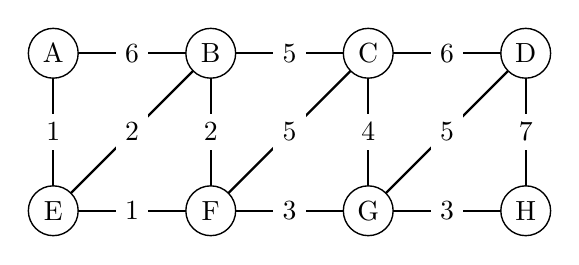
\begin{tikzpicture}
\Vertex[x=0,y=2]{A}
\Vertex[x=2,y=2]{B}
\Vertex[x=4,y=2]{C}
\Vertex[x=6,y=2]{D}
\Vertex[x=0,y=0]{E}
\Vertex[x=2,y=0]{F}
\Vertex[x=4,y=0]{G}
\Vertex[x=6,y=0]{H}
\Edge[label=$1$](A)(E)
\Edge[label=$6$](A)(B)
\Edge[label=$2$](B)(E)
\Edge[label=$2$](B)(F)
\Edge[label=$5$](B)(C)
\Edge[label=$5$](C)(F)
\Edge[label=$4$](C)(G)
\Edge[label=$6$](C)(D)
\Edge[label=$5$](D)(G)
\Edge[label=$7$](D)(H)
\Edge[label=$1$](E)(F)
\Edge[label=$3$](F)(G)
\Edge[label=$3$](G)(H)
\end{tikzpicture} \\
(a) What is the cost of its minimum spanning tree? \\\\
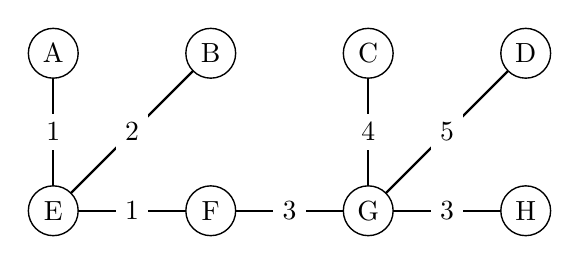
\begin{tikzpicture}
\Vertex[x=0,y=2]{A}
\Vertex[x=2,y=2]{B}
\Vertex[x=4,y=2]{C}
\Vertex[x=6,y=2]{D}
\Vertex[x=0,y=0]{E}
\Vertex[x=2,y=0]{F}
\Vertex[x=4,y=0]{G}
\Vertex[x=6,y=0]{H}
\Edge[label=$1$](A)(E)
\Edge[label=$2$](E)(B)
\Edge[label=$4$](C)(G)
\Edge[label=$5$](D)(G)
\Edge[label=$1$](E)(F)
\Edge[label=$3$](F)(G)
\Edge[label=$3$](G)(H)
\end{tikzpicture} \\
Cost = 19 \\
(b) How many minimum spanning trees does it have? \\
Other MST: \\\\
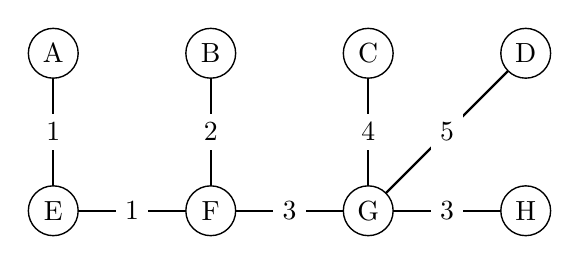
\begin{tikzpicture}
\Vertex[x=0,y=2]{A}
\Vertex[x=2,y=2]{B}
\Vertex[x=4,y=2]{C}
\Vertex[x=6,y=2]{D}
\Vertex[x=0,y=0]{E}
\Vertex[x=2,y=0]{F}
\Vertex[x=4,y=0]{G}
\Vertex[x=6,y=0]{H}
\Edge[label=$1$](A)(E)
\Edge[label=$2$](B)(F)
\Edge[label=$4$](C)(G)
\Edge[label=$5$](D)(G)
\Edge[label=$1$](E)(F)
\Edge[label=$3$](F)(G)
\Edge[label=$3$](G)(H)
\end{tikzpicture} \\
Answer: 2 MSTs \\
(c) Suppose Kruskal's algorithm is run on this graph. In what order are the edges added to the MST? For each edge in this sequence, give a cut that justifies its addition. \\
\begin{center}
\begin{tabular} { |c|c|c| }
\hline
Cut & Edge Added & Cost \\
\hline
\{\} & A & 0 \\ 
\hline
\{A\} & E & 1 \\
\hline
\{A,E\} & F & 1 \\
\hline
\{A,E,F\} & B & 2 \\
\hline
\{A,E,F,B\} & G & 3 \\
\hline
\{A,E,F,B,G\} & H & 3 \\
\hline
\{A,E,F,B,G,H\} & C & 4 \\
\hline
\{A,E,F,B,G,H,C\} & D & 5 \\
\hline
\{A,E,F,B,G,H,C,D\} & $\emptyset$ & 19 \\
\hline
\end{tabular}
\end{center}

\pagebreak

%%%%% PROBLEM 3 %%%%%

\section{Problem 3}
You are given a connected graph $G$ with $n$ vertices and $m$ edges, and a minimum spanning tree $T$ of the graph. Suppose one of the edge weights $c(e)$ for an edge $e \in T$ is updated. Give an algorithm that runs in time $O(m)$ to test if $T$ still remains the minimum spanning tree of the graph. You may assume that all edge weights are distinct both before and after the update. Explain why your algorithm runs in $O(m)$ time and is correct. \\\\
ALGORITHM: \\
Delete the updated edge $e=\{u,v\}$ from $T$, this gives us at most two disconnected cuts $S_1 \in T$ and $S_2 \in T$ where $u \in S_1$, $v \in S_2$ \\
For vertex $v \in S_2$: \\
\tab Pick an edge $f$ from updated $G$ with least attachment cost to $v$: $O(m)$ \\
\tab If $f = e$: $T$ still remains the MST. \\ 
\tab Else: $T$ is no longer the MST. \\\\
This algorithm runs in $O(m)$ time because finding a minimum edge $f \in G$ that connects to $v$ (after deleting $e$) will take at most $m$ iterations. This is because $v$ can be connected to at most $m$ other vertices in the graph $G$. All other operations in the algorithm run at $O(1)$ time, making the total runtime $O(m)+O(1)+O(1) = O(m)$. \\
This algorithm is correct because the deletion of $e=\{u,v\}$ from $T$ will create two cuts $S_1 \in T$ and $S_2 \in T$ in which $u \in S_1$ and $v \in S_2$. All that is necessary to create an MST from these two cuts is to find the minimum edge from $S_1$ to $S_2$ in the updated $G$. We do not need to find the minimum edge from the set of all $S_1$ vertices to the set of all $S_2$ vertices because the path from $v$ to the end of $S_2$ is guaranteed to be in correct MST order due to the \textbf{cut property}. For the same reason, all of the edges in $S_1$ will be in correct MST order. Thus, as long as we choose a minimum edge that connects a vertex in $S_1$ to $v \in S_2$, we are guaranteed to be left with a MST. 

\pagebreak

%%%%% PROBLEM 4 %%%%%

\section{Problem 4}
Given an undirected graph $G=(V,E)$, a subset of vertices $I \subset V$ is an independent set in $G$ if no two vertices in $I$ are adjacent to each other. Let $\alpha(G)=$max$\{|I|:I$ an independent set in $G\}$. Give an efficient algorithm for computing an independent set of maximum size in a tree. \\
Let $T=(V,E)$ be an acyclic graph on $n$ vertices.\\
(a) Prove that if $u$ is a leaf in $T$, then there is a maximum-size independent set in $T$ which contains $u$. That is, for every leaf in $u$, there is an independent set $I$ such that $u \in I$ and $|I|=\alpha(T)$.\\\\
LEMMA: For a vertex $v \in I$ that is not a leaf but is adjacent to at least one leaf, removing $v$ from $I$ and adding $v$'s leaves to $I$ still gives us a valid independent set. \\
PROOF: Since $T$ is acyclic, $v$ has at most one parent node and at least one leaf node $u$. \\
If we remove $v$ from $I$ and add $u$ to $I$, we still get a valid independent set because $u$ is adjacent only to $v$, which no longer appears in the set $I$. \\\\
PROOF BY CONTRADICTION: \\
Suppose there is a maximum independent set $I$ such that $|I|=\alpha(T)$ and the leaf $u \not\in I$. \\
Since $u$ is a leaf, this implies that there exists a vertex $v$ which is adjacent to $u$. \\
If $v \not \in I$, then $I$ could not have been the maximum independent set due to the fact that $u \not \in I$. \\
If $v \in I$, then $degree(v)\geq2$, since it is not a leaf. \\
Let $L$ be the set containing the leaves of $v$, where $u \in L$. \\
$|L|\geq1$, since $degree(v)\geq2$. \\
By the lemma above, we can remove $v$ from $I$ and add the vertices in the set $L$ to the set $I$. \\
Since $|L|\geq1 \rightarrow |I \cup L|\geq|I|$. \\
$\therefore$ The original set $I$ could not have been the maximum-size  independent set in $T$ if $L>1$. \\
$\therefore$ There exists an independent set $I$ such that $u \in I$ and $|I|=\alpha(T)$. 

\pagebreak
(b) Given the graph $T$ as input (in adjacency edge representation), give an algorithm to compute an independent-set of maximum size, $\alpha(T)$, in $T$. Your algorithm should run in time $O(|V|*|E|)$, prove correctness of your algorithm. \\\\
We can use dynamic programming to find the maximum independent set. \\
Let $OPT(T)$ denote the maximum independent set of $T$. \\
Let $OPT(\emptyset)=0$. \\
1. Label each vertex in $T$ from $\{1, 2, 3, \dots, n\}$. \\
2. Let the vertex labeled $s$ be the last vertex in the $T$ visited using some traversal algorithm (like DFS). \\
3. Let $A[s]$ denote the list of neighbors of $s$. \\
4. We observe that $I$ can either contain the vertex $s$ or not contain $s$: \\
\tab If $s \in I: OPT(T) = (1 + OPT(T-A[s]))$ \\
\tab Else if $s \not \in I: OPT(T) = OPT(T-\{s\})$ \\
5. We can memoize $OPT(T)$ by having an $n$ length array $M$ that stores $1$ for every vertex in $T$ that appears in $I$, and stores $0$ otherwise. \\\\
FULL ALGORITHM: \\
Initialize array $M$ of length $n$ where all entries are $0$. \\
Max-Independent-Set-Opt($T$): \\
\tab If $M[T]$ is empty and $n=0$ or $1$: \\
\tab \tab $M[T] = n$ \\
\tab Else: \\
\tab \tab $M[T]=$max$(1+M[T-A[s]], M[T-\{s\}])$ \\
\tab Return $M[T]$ \\\\
PROOF BY INDUCTION: \\
BASE CASE: $n=0$, $T=\emptyset$, $I=\emptyset$, $|I|=0$. \\
INDUCTION: Suppose the algorithm works for $n=0$, show that it works for $n+1$: \\
\tab Let $OPT(T)$ be the optimal solution that returns $\alpha(T)$. \\
\tab Suppose we add 1 vertex $v$ to $T$. The optimal solution would then become $OPT(T+\{v\})$. \\
\tab Since $OPT(T)$ was already the optimal solution, adding $v$ will have two possibilities: $v$ will be included in the set $I$ or $v$ will not be included in the set $I$. \\
\tab CASE 1: $v \in I$: \\
\tab \tab If $v$ is added to $I$, all of $v$'s neighbors must not be in $I$. The addition of $v$ is represented by $+1$ and the removal of $v$'s neighbors is represented by $T-A[v]$, so the resulting optimal solution is $OPT(T+\{v\})=(1+OPT(T-A[v]))$. \\
\tab CASE 2: $v \not \in I$: \\
\tab \tab If $v$ is not added to $I$, we only need the optimum solution to the remaining vertices, i.e. $T$ with $v$ removed from it. This is represented by $T-\{v\}$, so the resulting optimal solution is $OPT(T+\{v\})=OPT(T-\{v\})$. \\
\tab We take the maximum value of either case to be $\alpha(T)$. \\
$\therefore$ The algorithm is correct, since the two possible cases are handled correctly. \\


\end{document}